\documentclass[12pt,english,hyperfootnotes=false,hidelinks]{article}

%%%% Packages
\usepackage{lmodern}
\usepackage{tablefootnote}
\usepackage[T1]{fontenc}
\usepackage[latin9]{inputenc}
\usepackage{geometry}
\geometry{verbose,tmargin=1.25in,bmargin=1.25in,lmargin=1.25in,rmargin=1.25in}
\usepackage{float}
\usepackage{amsmath}
\usepackage{graphicx}
\usepackage{setspace}
\usepackage[authoryear]{natbib}
\usepackage[bottom,multiple]{footmisc}
\usepackage{geometry}
\usepackage{adjustbox}
\usepackage[hyphenbreaks]{breakurl}
\usepackage{booktabs}
\usepackage{pdflscape}
\usepackage{siunitx}
\usepackage{numprint}
\usepackage{threeparttable}
\usepackage{caption}
\usepackage{babel}
\usepackage{xcolor}
\usepackage{longtable}
\usepackage{afterpage}
\usepackage{dcolumn}
\usepackage{multicol}
\usepackage{amsfonts}
\usepackage{adjustbox}
\usepackage{xurl}
\usepackage{hyperref}
\usepackage{catchfilebetweentags}
\usepackage{csquotes}
\usepackage{framed}
\usepackage{multirow}
\usepackage{tikz}
\usetikzlibrary{decorations.pathreplacing}
% define check and xmark
\usepackage{pifont}
\newcommand{\cmark}{\ding{51}}%
\newcommand{\xmark}{\ding{55}}%

%%%% Other settings
\captionsetup[table]{skip=0pt}
\interfootnotelinepenalty=10000
\newcolumntype{R}[1]{>{\raggedright\let\newline\\\arraybackslash\hspace{0pt}}m{#1}}
\newcolumntype{C}[1]{>{\centering\arraybackslash}m{#1}}

\newtheorem{assumption}{Assumption}

%%% Command for extracting numbers
\newcommand{\gn}[1]{\ExecuteMetaData[results/results.tex]{#1}}



\title{
Bureaucratic Capacity and Urban Planning: Evidence from Los Angeles
\thanks{
This project was supported in part by the UCLA Ziman Center for Real Estate Research. We thank the Ziman Center for its financial support. We also thank Ignacio Ramirez for his invaluable research assistance. The views expressed in this paper are solely those of the authors and do not necessarily reflect those of the Ziman Center. All errors are our own.
}
}

\author{
    Stuart Gabriel\thanks{UCLA Anderson School of Management, 110 Westwood Plaza, Suite C412, Los Angeles, CA 90095-1481;  stuart.gabriel@anderson.ucla.edu} \and
    Matthew Histen\thanks{California State University, Northridge, David Nazarian College of Business and Economics, 18111 Nordhoff St, Northridge, CA 91330; matthew.histen@csun.edu} \and
    Edward Kung\thanks{Corresponding Author: California State University, Northridge, David Nazarian College of Business and Economics, 18111 Nordoff St, Northridge, CA 91330; edward.kung@csun.edu}
}

\date{\today}

\begin{document}

\maketitle

\singlespacing

\vspace{-1cm}

\begin{abstract}
Lorem ipsum dolor sit amet, consectetur adipiscing elit, sed do eiusmod tempor incididunt ut labore et dolore magna aliqua. Ut enim ad minim veniam, quis nostrud exercitation ullamco laboris nisi ut aliquip ex ea commodo consequat. Duis aute irure dolor in reprehenderit in voluptate velit esse cillum dolore eu fugiat nulla pariatur. Excepteur sint occaecat cupidatat non proident, sunt in culpa qui officia deserunt mollit anim id est laborum.
\end{abstract}


\noindent{\textit{Keywords}: local land-use regulation, bureaucratic efficiency} \\
\noindent {\textit{JEL} Classification: D73, R14, R38, R52.} \\


\doublespacing

\pagebreak


\section{Introduction}\label{sec_intro}

Lorem ipsum dolor sit amet, consectetur adipiscing elit, sed do eiusmod tempor incididunt ut labore et dolore magna aliqua. Ut enim ad minim veniam, quis nostrud exercitation ullamco laboris nisi ut aliquip ex ea commodo consequat. Duis aute irure dolor in reprehenderit in voluptate velit esse cillum dolore eu fugiat nulla pariatur. Excepteur sint occaecat cupidatat non proident, sunt in culpa qui officia deserunt mollit anim id est laborum.
\section{Data}\label{sec_data}

\subsection{Institutional Background}

The Los Angeles planning and approvals process for urban development is a multi-layered process that requires the input of multiple agencies. 


\subsection{Data Acquisition}

The Los Angeles Planning Department's website maintains robust public documentation of City Planning Commission Meetings. For each meeting, the agenda, minutes, and any supplemental documents relevant to the meeting (letters from the public, traffic assessments, architectural reports, etc.) are available for download as PDF files.\footnote{As of August 26th, 2025, these documents are available at the URL: \url{https://planning.lacity.gov/about/commissions-boards-hearings}.} We downloaded these documents for all City Planning Commission meetings from May 10th, 2018 to December 19th, 2024. This resulted in documentary data for \gn{NumberOfMeetings} meetings, covering \gn{NumberOfAgendaItems} agenda items, with \gn{NumberOfSupplementalDocs} supplemental documents, spanning \gn{PageCount} pages of PDF documents. Download occurred on April 10th, 2025.

Since we are primarily interested in bureaucratic decision making, we limit our attention to the agenda items that require a decision from the board. These are identified by agenda items titled according to their Planning Department case numbers, which have a standardized format of ``[CASE PREFIX]-[YEAR]-[SERIAL NUMBER]-[CASE SUFFIXES]''. Other agenda items include items like ``Director's Report'' and ``General Public Comment'' which do not require any decisions on the part of the board. Altogether, there were \gn{NumberOfCases} agenda items requiring a decision from the board, as identified by their Planning Department case numbers.

A typical agenda item is a request from a developer to approve a development plan that goes beyond what the site's zoning designation would allow, or an appeal of a previously approved plan. Figure \ref{fig_example_agenda_item} shows an example of an agenda item. The case number is DIR-2019-6048-TOC-SPR-WDI-1A. This was a project that was initially approved by the Director of Planning (DIR). The project was granted bonuses under the Los Angeles Transit Oriented Communities program (TOC), the project requires a site plan review (SPR), and the project was granted a waiver of dedications and improvements (WDI). However, this previously approved plan was appealed (1A), and the appeal is now to be considered by the City Planning Commission. In addition to the information contained in the case number, the agenda shows additional information such as the Council District that the project is located in, and other specific details about the project proposal.

Figure \ref{fig_example_minutes_item} shows the associated minutes for the agenda item shown in Figure \ref{fig_example_agenda_item}. From the minutes, we can see that the appeal was granted in part and denied in part. The CPC upheld the Director of Planning's previous decision, but additional conditions were applied, thus allowing the project to move forward as long as the developer adheres to the new conditions. This outcome, the partial granting of an appeal or the approval of a project with modifications, is common but not the only kind of outcome. Sometimes, the requested actions by the developer are granted in their entirety without additional conditions or modifications. Rarely, the requested actions are denied entirely. A more common occurrence than denial is that the CPC puts the decision off to a later date. We will discuss the distribution of motion outcomes and voting patterns later in Section \ref{sec_descriptive_statistics}.

Figures \ref{fig_example_support_letter} and \ref{fig_example_oppose_letter} show examples of letters submitted by the public in support of and in opposition to the above project. The support letter emphasizes how the project will ease traffic, reduce air pollution, and increase housing availability. The opposition letter emphasizes concerns about displacement and how the proposed units will be unaffordable to current residents of the neighborhood. These letters typify the kinds of concern expressed by community residents in this dataset; however, the number of letters that this project attracted is atypical (DIR-2019-6048 just happens to be a particularly controversial project). We will discuss the distribution of support and opposition letters across projects later in Section \ref{sec_descriptive_statistics}.

\subsection{Data Extraction}

The documentary data provides a wealth of information about CPC cases and their outcomes. However, the information is locked within textual data that is difficult to process using traditional methods. For example, traditional NLP methods based on token and pattern matching would have a hard time comparing the agenda to the minutes and determining whether the requested actions were approved, partially approved, approved with conditions, denied, or whether the decision was postponed to a future date. 

To extract usable features from the textual content more robustly, we make use of OpenAI's \texttt{gpt-4o} generative language model. For example, the model can be asked to read the text of the agenda, read the text of the minutes, and explain what the result of committee's proposed motion was in terms of its implications for the development project---was the project approved, partially approved or approved with conditions, denied, or was the decision postponed? The methodology and prompts we used to perform the data extraction are described in detail in Appendix \ref{sec_data_appendix}. In this section, we will instead focus on the data features that were extracted from the text.

\paragraph{Agenda items.} For each agenda item, we extracted the following information from the text: 
\begin{itemize}[noitemsep, topsep=0pt]
\item Item number (used primarily for identification);
\item Item title (for cases requiring a decision, this is always a Planning Department case number)
\item Short AI-generated summary of the agenda item's content;
\item The Council District(s) to which the item applies
\end{itemize}

\paragraph{Minutes.} For each agenda item, we extract the following information from its minutes text:
\begin{itemize}[noitemsep, topsep=0pt]
\item Short AI-generated summary of the deliberations and the motion that was ultimately voted on;
\item Implication of the motion for the proposed project: were the requested actions approved, approved in part or with conditions and modifications, denied, or were deliberations continued to a future date?
\item Result of the vote (whether the motion passed or failed)\footnote{Note that a motion passing is not the same as a project getting approved, nor is a motion failing the same as a project getting denied. A Member may move to deny the project's requested actions, or move to accept an appeal of a previously approved project, in which case the motion passing implies a denial of the project. These nuances highlight why LLMs are helpful in the data extraction process.};
\item Vote tallies: the number of ayes, nays, absences, abstentions, and recusals.
\end{itemize}

\paragraph{Supplemental documents.} For each supplemental document, we extract the following information from its text:
\begin{itemize}[noitemsep, topsep=0pt]
\item Type of document: whether it is a letter or petition, a technical modification or procedural matter, a scientific or technical report (traffic, environmental, etc), or a credentials document (CV, resume, biography, etc); 
\item Type of author: whether the author of the document is an individual, an advocacy group, a consultant, a lawyer, a developer, or a public official;
\item Which agenda item(s) it references;
\item Short AI-generated summary of the document contents;
\item Support or opposition: Whether the document definitely supports, somewhat supports, is neutral towards, somewhat opposes, or definitely opposes the referenced agenda item(s).
\end{itemize}

~

\noindent The resulting dataset contains \gn{NumberOfCases} agenda items with motions voted on by the CPC. Table \ref{tab_result_unanimity} shows the distribution of the motion outcomes by the unanimity of the vote. Two important facts emerge about the CPC process. First, a minuscule number of projects are denied outright (\gn{CasesDeniedPct} of all cases). Rather than being denied, a more common occurrence is that the decision is postponed to a later date (\gn{CasesContinuedPct} of cases) or the requested actions are only partially approved or approved with conditions or modifications (\gn{CasesApprovedWithModsPct} of cases). Second, most decisions were unanimous (\gn{CasesUnanimousPct} of all cases). Because of these two facts, we do not view disagreement \emph{within} the board as a significant source of friction in moving development projects through the pipeline. Moreover, few projects are denied outright, so the impact of CPC hearings on final outcomes must come through either i) a slowing down of the process due to having to wait for the decision, which itself may be delayed multiple times; or ii) changes to the project plan that potentially add cost or time to the development, or which could  dissuade the developer from even moving forward with the project. Our primary analysis will therefore focus on the bureaucratic factors which lead to either delayed decision making or attaching conditions and modifications to the project proposal.




%\bibliographystyle{aer}
%\bibliography{81refs}

%\pagebreak

\pagebreak

\begin{figure}[H]
\caption{Example of an Agenda Item} \label{fig_example_agenda_item}
\vspace{-0.5cm}
\begin{center}
\fbox{
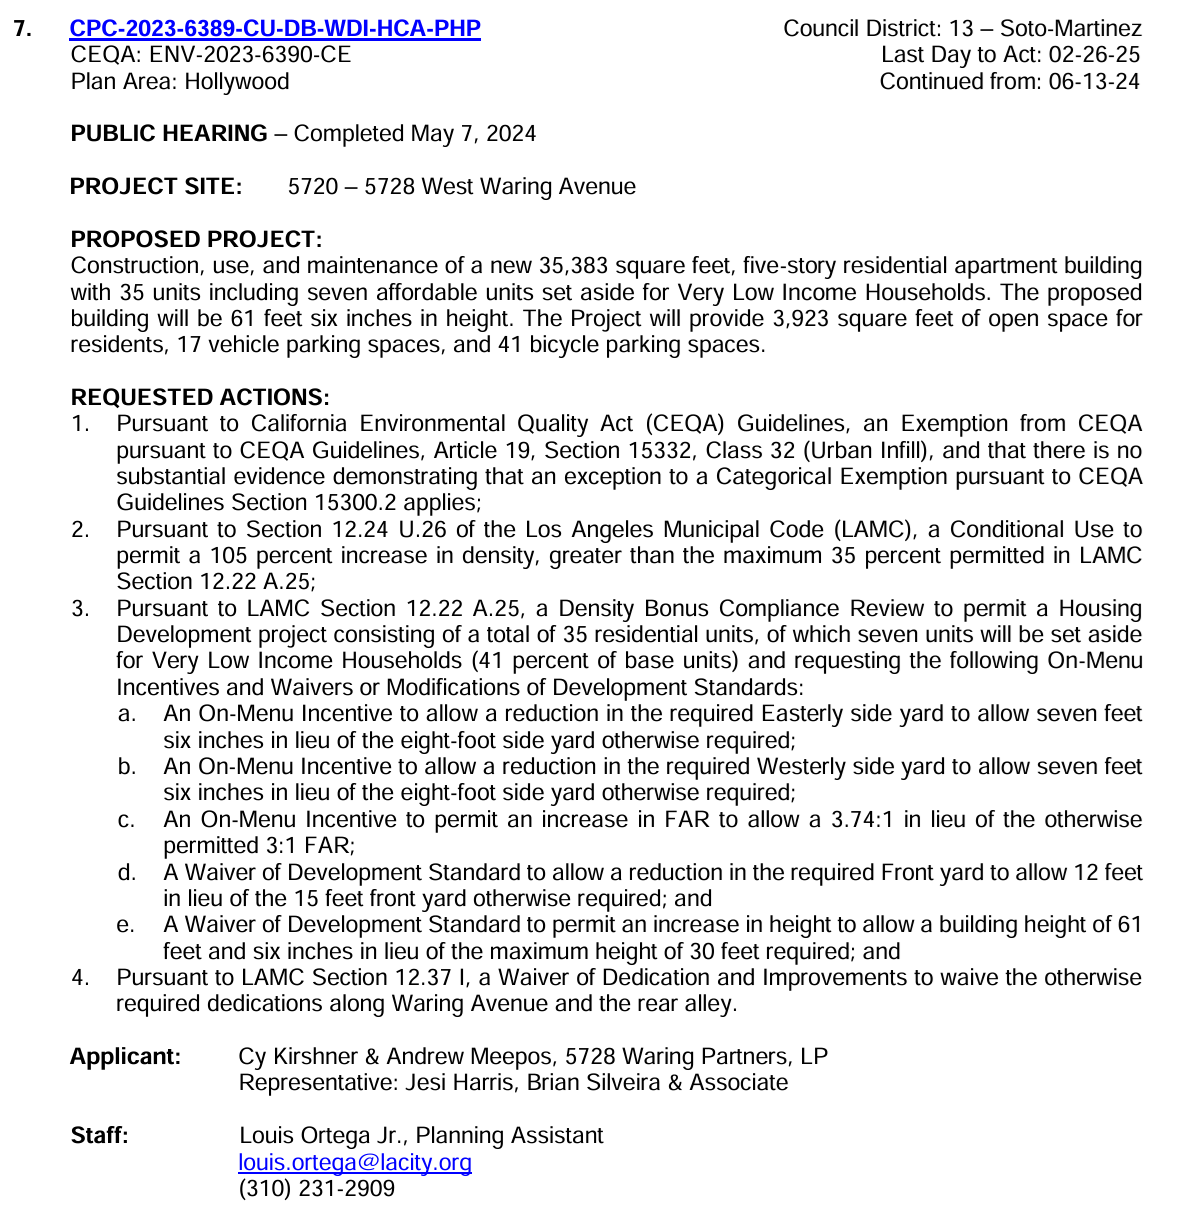
\includegraphics[width=\textwidth]{figures/example-agenda-item.png}
}
\end{center}
\end{figure}

\pagebreak

\begin{figure}[H]
\caption{Example of a Minutes Item} \label{fig_example_minutes_item}
\vspace{-0.5cm}
\begin{center}
\fbox{
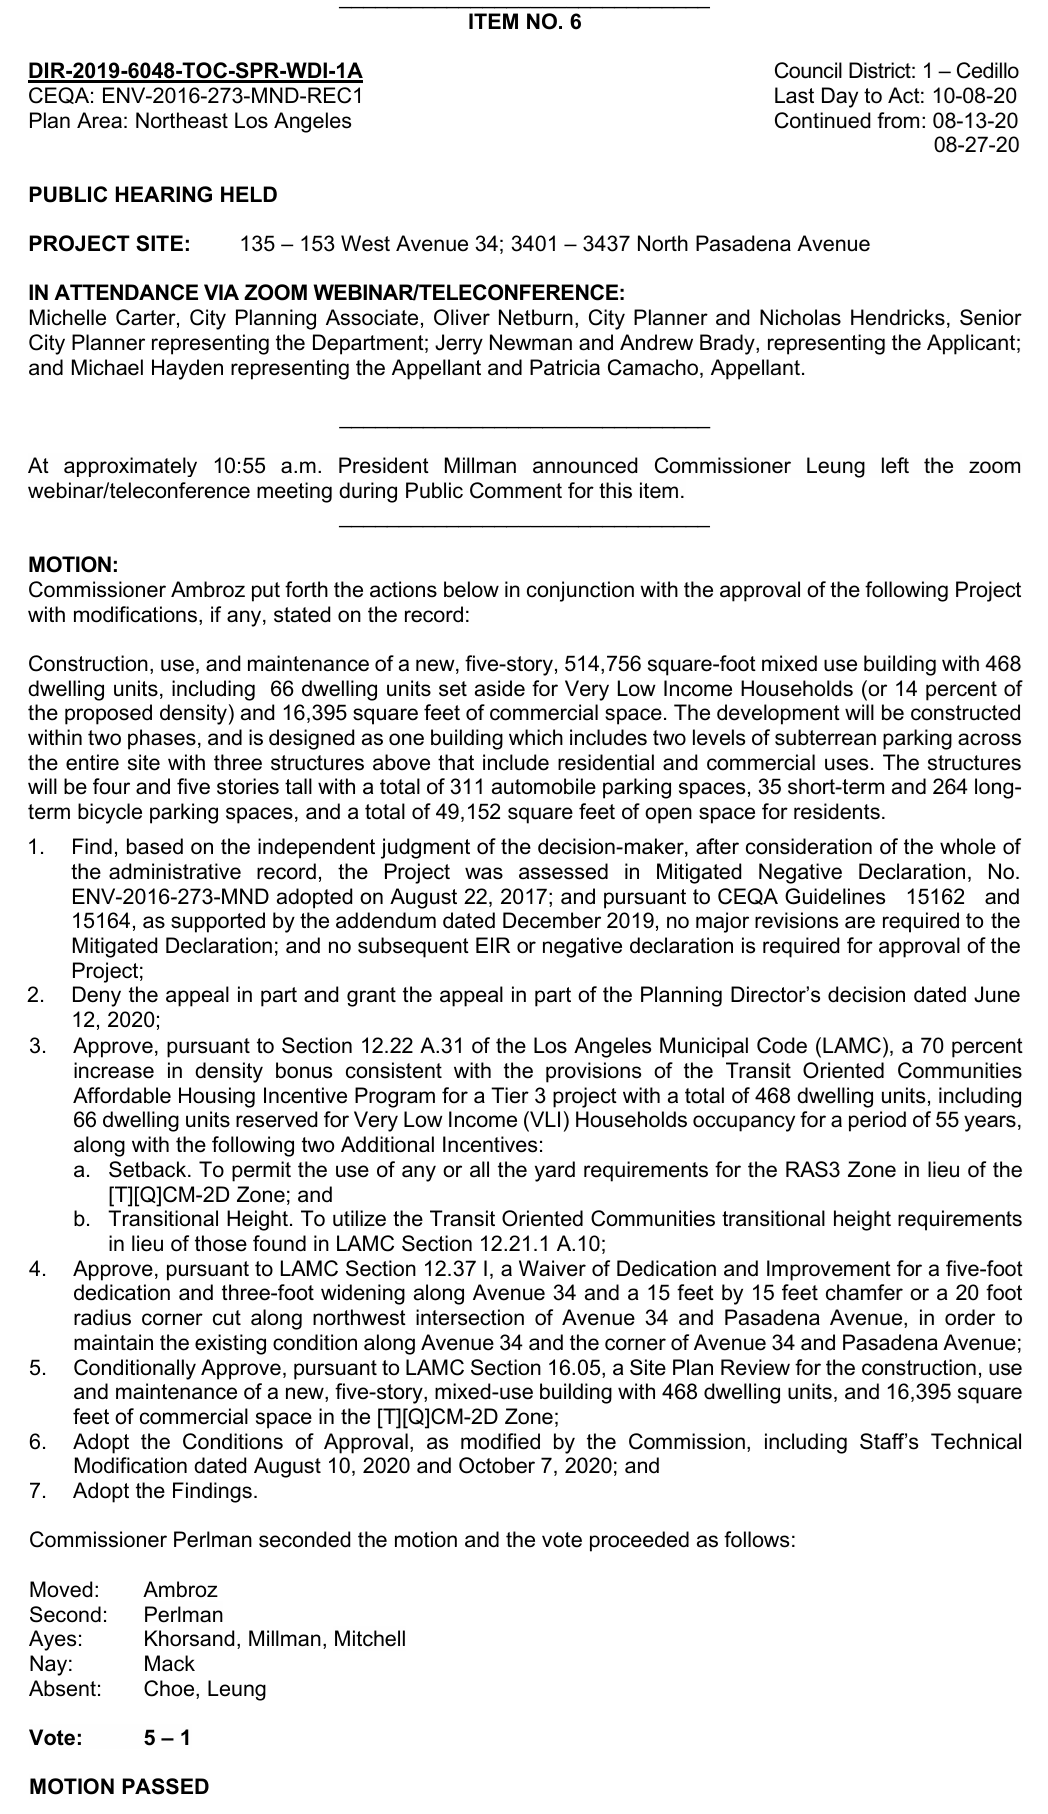
\includegraphics[height=0.95\textheight]{figures/example-minutes-item.png}
}
\end{center}
\end{figure}

\pagebreak

\begin{figure}[H]
\caption{Example of a Support Letter} \label{fig_example_support_letter}
\vspace{-0.5cm}
\begin{center}
\fbox{
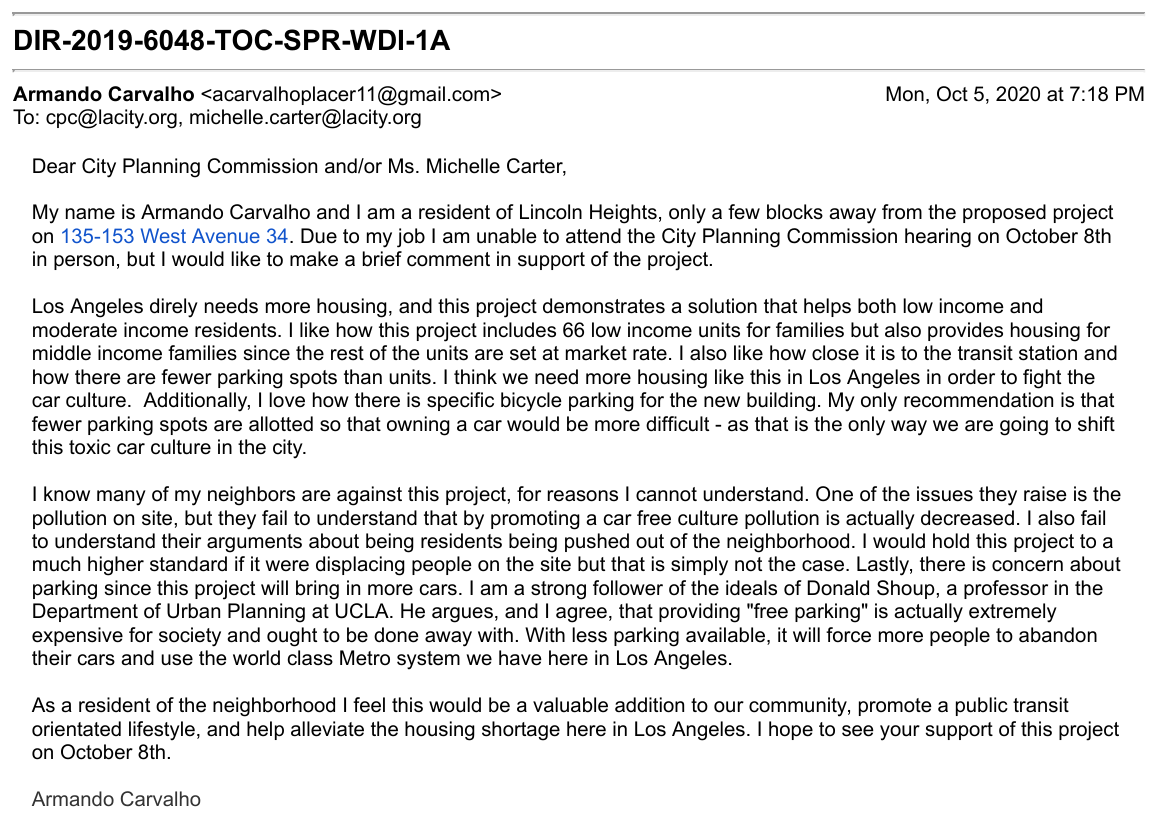
\includegraphics[width=\textwidth]{figures/example-support-letter.png}
}
\end{center}
\end{figure}

\pagebreak

\begin{figure}[H]
\caption{Example of an Oppose Letter} \label{fig_example_oppose_letter}
\vspace{-0.5cm}
\begin{center}
\fbox{
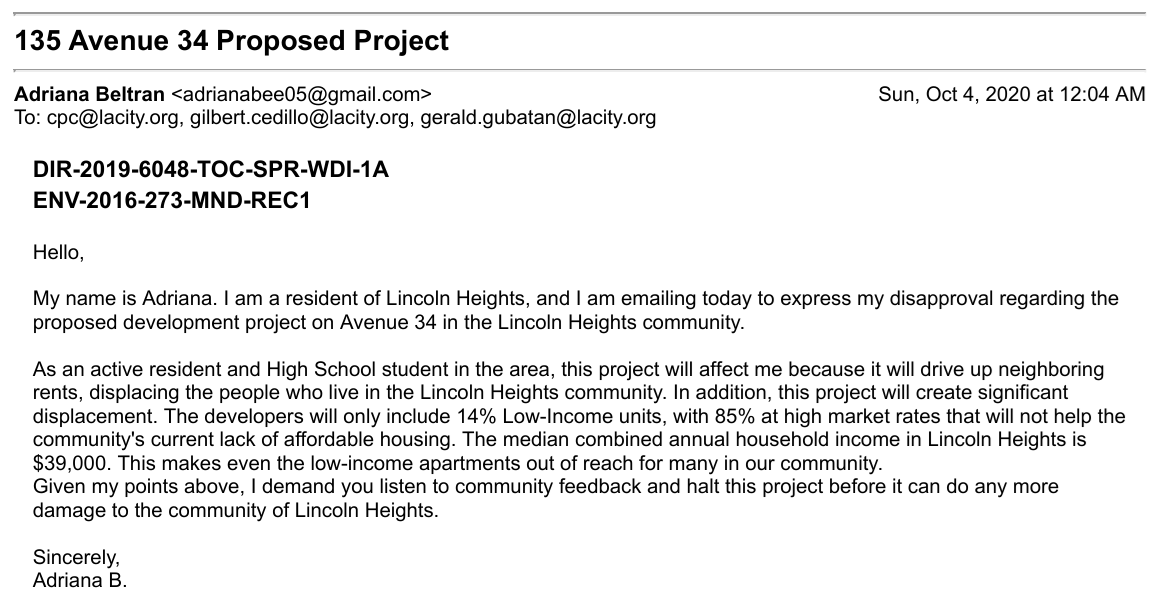
\includegraphics[width=\textwidth]{figures/example-oppose-letter.png}
}
\end{center}
\end{figure}

\pagebreak

\begin{table}[H]
\caption{Summary of Vote Results}
\vspace{0.2cm}
\label{tab_result_unanimity}
\begin{adjustbox}{max width=\textwidth}
\begin{threeparttable}
\begin{tabular}{lrrrrr} \toprule
 & \multicolumn{3}{c}{Unanimity} &  & \\ \cline{2-4} 
 & Unanimous & 1 Nay & >1 Nays & \multicolumn{2}{c}{Total} \\ \midrule
\textit{Project Implication} & & & & & \\ 
~ ~ APPROVED & 365 & 23 & 4 & 392 & (53.9\%) \\ [1ex] 
~ ~ APPROVED IN PART OR WITH MODIFICATIONS & 183 & 17 & 16 & 216 & (29.7\%) \\ [1ex] 
~ ~ DELIBERATIONS CONTINUED TO FUTURE DATE & 108 & 4 & 0 & 112 & (15.4\%) \\ [1ex] 
~ ~ DENIED & 5 & 0 & 2 & 7 & (1.0\%) \\ [1ex] 
~ ~ TOTAL & 661 & 44 & 22 & 727 &  \\ [1ex] 
 & (90.9\%) & (6.1\%) & (3.0\%) &  &  \\ [1ex] 
\end{tabular}

\begin{tablenotes}
\item {\textit{Notes: } Notes.}
\end{tablenotes}
\end{threeparttable}
\end{adjustbox}
\end{table}

\pagebreak

\appendix
\renewcommand{\thefigure}{A\arabic{figure}}

\section{Data Appendix} \label{sec_data_appendix}

\subsection{Data Extraction with LLMs}

Extracting data from the raw PDFs downloaded from the Planning Department website is a multi-step process. First, individual agenda items need to be extracted from the raw agenda PDF. This is difficult using traditional NLP methods because the boundaries between agenda items in the PDF are not always consistently demarcated. However, LLMs are quite suited to this task of identifying the unique agenda items out of a single PDF containing the agenda.

The first step, therefore, is to extract the individual agenda items. Figure \ref{fig_split_agenda_prompt} shows the prompt we used to have the LLM read the agenda, then extract each individual agenda item. We ask the LLM to return the agenda's item number, its title (which is a Planning Department case number for any items requiring a decision), and a short summary of the agenda item.

After the agenda items are extracted, the next step is to extract data about each agenda item, using the agenda text. The raw agenda PDF is split into its individual components based on the extracted item number and title for each agenda item. The text for each individual agenda item is then fed into the prompt shown in Figure \ref{fig_agenda_items_prompt}. The outputted response is then used to extract the data features listed in Section \ref{sec_data}.

After extracting data from the agenda text, we extract information about the deliberations over each agenda item from the minutes text. We first split the minutes PDF into the components relevant to each individual item, using the item number and title. We then take the agenda text for that item and the minutes text for that item and feed it into the prompt shown in Figure \ref{fig_minutes_prompt}. The response from the LLM is then processed to extract the data features.

Lastly, we 





\pagebreak

\begin{figure}[H]
\caption{Prompt to Split and Summarize Agenda} \label{fig_split_agenda_prompt}
\vspace{-0.5cm}
\begin{center}
\fbox{
\begin{minipage}{0.9\textwidth}
\texttt{
The following extracted PDF text contains the agenda for a LA City Planning Commission meeting. \\ 
\\ 
For each agenda item, return a summary in the following format:\\ 
\\ 
ITEM NO: <agenda item number>\\ 
TITLE: <title of agenda item>\\ 
SUMMARY: <short summary of agenda item>\\ 
\\ 
Separate each response by "------"\\ 
\\ 
AGENDA:\\ 
\\ 
[AGENDA TEXT]
}
\end{minipage}
}
\end{center}
\end{figure}



\end{document}

